\documentclass{article}

\usepackage{amsmath}
\usepackage[utf8]{inputenc}
\usepackage{amssymb}
\usepackage{geometry}
\usepackage{fancyhdr}
\usepackage{tikz}
\usepackage{mdframed}
\usepackage{xcolor}
\usepackage[unicode=true, colorlinks=true, linkcolor=black, urlcolor=blue, citecolor=blue]{hyperref}

\definecolor{lightorange}{HTML}{f7d6e0}
% Define the question environment
\newenvironment{question}
{\begin{mdframed}[backgroundcolor=white]}
{\end{mdframed}}

% Define the solution environment
\newenvironment{solution}
{\begin{mdframed}[backgroundcolor=lightorange,hidealllines=true]}
{\end{mdframed}}

% Page setup
\geometry{a4paper, margin=2cm}
\pagestyle{fancy}
\fancyhf{}
\lhead{I2 Review}
\rhead{\today}

\begin{document}

\begin{titlepage}
    \centering
    \vspace*{2cm}
    {\Huge\bfseries Optimizacion - I2}\\[1cm]
    \vspace{1cm}
    {\Large Nombre: \par}
    {\large Sebastian Lorca\par}
    \vspace{0.5cm}
    {\Large Date: \par}
    {\large \today \par}
    \vspace{0.5cm}
    {\Large Profesor: \par}
    {\large Raimundo Cuadrado\par}
    \vspace{0.5cm}
    {\Large Pontificia Universidad Católida de Chile\par}
    {\large Escuela de Ingeniería\par}
    \vspace{0.5cm}
    {\Large Departmento: \par}
    {\large Industrial\par}
    \vspace{0.5cm}
    {\Large Email: \par}
    {\large \href{mailto:sdlorca@uc.cl}{sdlorca@uc.cl}\par}
    \vspace{0.5cm}
    {\Large Sigla: \par}
    {\large ICS1113\par}
    \vspace{0.5cm}
    {\Large Semestre: \par}
    {\large 1/2024\par}
    \vspace{1cm}
\end{titlepage}
\tableofcontents
\newpage


\section{Modelación}

\subsection{Metodología}

\begin{enumerate}
    \item Entender el problema.
    \item Anotar toda la información relevante
    \begin{enumerate}
        \item Parámetros.
        \item Unidades de medida.
    \end{enumerate}
    \item Definir las variables de decisión.
    \item Construir restricciones (incluyendo NV\footnote{Naturaleza de las variables}).
    \item Si no se puede escribir una restricción, volver a (3).
\end{enumerate}

\subsection{Problemas Comunes}
\subsubsection{El Problema de la Mochila}

El problema de la mochila busca maximizar el valor de los objetos que se pueden llevar en una mochila, dada una capacidad máxima. La formulación matemática es la siguiente:

\begin{align*}
    \text{Maximizar} \quad & \sum_{i=1}^{n} v_i x_i \\
    \text{Sujeto a} \quad & \sum_{i=1}^{n} w_i x_i \leq W \\
    & x_i \in \{0, 1\} \quad \forall i \in \{1, \ldots, n\}
\end{align*}

\subsubsection{El Problema de la Asignación}

El problema de la asignación busca asignar $n$ trabajadores a $n$ tareas, de manera que se minimice el costo total. La formulación matemática es la siguiente:

\begin{align*}
    \text{Minimizar} \quad & \sum_{i=1}^{n} \sum_{j=1}^{n} c_{ij} x_{ij} \\
    \text{Sujeto a} \quad & \sum_{i=1}^{n} x_{ij} = 1 \quad \forall j \in \{1, \ldots, n\} \\
    & \sum_{j=1}^{n} x_{ij} = 1 \quad \forall i \in \{1, \ldots, n\} \\
    & x_{ij} \in \{0, 1\} \quad \forall i, j \in \{1, \ldots, n\}
\end{align*}

\subsubsection{El Problema de la Ruta más Corta}

El problema de la ruta más corta busca encontrar la ruta más corta entre dos nodos en un grafo. La formulación matemática es la siguiente:

\begin{align*}
    \text{Minimizar} \quad & \sum_{(i, j) \in A} c_{ij} x_{ij} \\
    \text{Sujeto a} \quad & \sum_{j \in N} x_{ij} - \sum_{j \in N} x_{ji} = 
    \begin{cases}
        -1 & \text{si } i = 1 \\
        1 & \text{si } i = n \\
        0 & \text{en otro caso}
    \end{cases} \quad \forall i \in N \\
    & x_{ij} \in \{0, 1\} \quad \forall (i, j) \in A
\end{align*}

\subsection{Problema del Vendedor Viajero (TSP)}

El problema del vendedor viajero busca encontrar el ciclo hamiltoniano de menor costo en un grafo completo. La formulación matemática es la siguiente:

\begin{align*}
    \text{Minimizar} \quad & \sum_{(i, j) \in A} c_{ij} x_{ij} \\
    \text{Sujeto a} \quad & \sum_{i \in N} x_{ij} = 1 \quad \forall j \in N \\
    & \sum_{j \in N} x_{ij} = 1 \quad \forall i \in N \\
    & u_i - u_j + n x_{ij} \leq n - 1 \quad \forall i, j \in N, j \neq 1, i \neq 1 \\
    & 2 \leq u_i \leq n \quad \forall i \in N \\
    & x_{ij} \in \{0, 1\} \quad \forall (i, j) \in A
\end{align*}

\subsection{Problemas en Redes}

\subsubsection{Flujo Máximo}

El problema de flujo máximo busca maximizar el flujo de una red, dada una capacidad en cada arco. La formulación matemática es la siguiente:

\begin{align*}
    \text{Maximizar} \quad & f \\
    \text{Sujeto a} \quad & 0 \leq f_{ij} \leq u_{ij} \quad \forall (i, j) \in A \\
    & \sum_{j \in N} f_{ij} - \sum_{j \in N} f_{ji} = 
    \begin{cases}
        -f & \text{si } i = 1 \\
        f & \text{si } i = n \\
        0 & \text{en otro caso}
    \end{cases} \quad \forall i \in N
\end{align*}

\subsubsection{Flujo a Costo Mínimo}

El problema de flujo a costo mínimo busca minimizar el costo de enviar un flujo de una fuente a un sumidero, dada una capacidad en cada arco. La formulación matemática es la siguiente:

\begin{align*}
    \text{Minimizar} \quad & \sum_{(i, j) \in A} c_{ij} f_{ij} \\
    \text{Sujeto a} \quad & 0 \leq f_{ij} \leq u_{ij} \quad \forall (i, j) \in A \\
    & \sum_{j \in N} f_{ij} - \sum_{j \in N} f_{ji} = 
    \begin{cases}
        -f & \text{si } i = 1 \\
        f & \text{si } i = n \\
        0 & \text{en otro caso}
    \end{cases} \quad \forall i \in N
\end{align*}
\subsubsection{Árbol de Expansión Mínima}

El problema del árbol de expansión mínima busca encontrar el árbol de expansión mínima en un grafo. La formulación matemática es la siguiente:

\begin{align*}
    \text{Minimizar} \quad & \sum_{(i, j) \in A} c_{ij} x_{ij} \\
    \text{Sujeto a} \quad & \sum_{i \in N} x_{ij} = 1 \quad \forall j \in N \\
    & \sum_{j \in N} x_{ij} = 1 \quad \forall i \in N \\
    & x_{ij} \in \{0, 1\} \quad \forall (i, j) \in A
\end{align*}

\section{Teoría y Conceptos}

\subsection{Convexidad}

\subsubsection{Combinación Convexa}

Una combinación convexa de un conjunto de puntos es una combinación lineal de esos puntos, donde los coeficientes son no negativos y suman 1.

\subsubsection{Conjunto Convexo}

Un conjunto es convexo si para cualquier par de puntos en el conjunto, la línea que los une está contenida en el conjunto.

\subsubsection{Función Convexa}

Una función es convexa si su dominio es un conjunto convexo y para cualquier par de puntos en el dominio, la línea que los une está por debajo de la función.

\subsubsection{Mínimo Global y Local}

Un punto $x$ se dice \textbf{mínimo global} de $f$ en $D$, (y solución óptima del problema P) si:

\begin{equation*}
    f(x) \leq f(y) \quad \forall y \in D
\end{equation*}

Un punto $x$ se dice \textbf{mínimo local} de $f$ en $D$ si existe un vecindario de $x$ en el que:

\begin{equation*}
    f(x) \leq f(y) \quad \forall y: \lVert x - y \rVert < \delta, y \in D
\end{equation*}

Si una función es convexa, cualquier mínimo local es un mínimo global.

\subsection{Existencia de Soluciones}

Todo $x \in D$ define una solución factible de $P)$. 

\subsubsection{Teorema 1: Existencia de Soluciones Óptimas de la Hipótesis H}

Sea

\begin{align*}
    \text{Minimizar} \quad & f(x) \\
    \text{Sujeto a} \quad & x \in D
\end{align*}

Si $f(x)$ es continua sobre $D$ y $D$ es cerrado y no vacío sobre $\mathbb{R}^n$, entonces bajo la hipótesis:

\begin{equation*}
    \text{H)} f(x) \rightarrow +\infty \quad \text{cuando } \lVert x \rVert \rightarrow +\infty
\end{equation*}

existe al menos una solución óptima de $P$. ($f(x)$ es coercitiva).

Un conjunto cerrado contiene a todos los puntos frontera. El caso de $D=\mathbb{R}^n$ es cerrado, ya que el conjunto de puntos frontera es vacío, y todo conjunto contiene al conjunto vacío.

\subsubsection{Teorema 2: Bolzonaro-Weierstrass}

Si $f$ es continua sobre un dominio \textbf{compacto y no vacío}, entonces el problema necesariamente tendrá solución óptima, ya que la imagen de $f$ también será compacta.

\subsubsection{Teorema 3: Soluciones Óptimas de la Programación Lineal}

En un problema lineal, si el dominio $D$ es vacío y cerrado, y la función objetivo está acotada inferiormente (para $\min$), entonces $P)$ tiene solución óptima.

\subsection{Teoría Poliedral}

\subsubsection{Poliedro}

Un poliedro es un conjunto de la forma:

\begin{equation*}
    P = \{x \in \mathbb{R}^n: Ax \leq b\}
\end{equation*}

donde $A \in \mathbb{R}^{m \times n}$ y $b \in \mathbb{R}^m$.

A los poliedros acotados se les llama \textbf{polítopos}.

\subsubsection{Cono}

Un cono es un conjunto de la forma:

\begin{equation*}
    C = \{x \in \mathbb{R}^n: Ax \leq 0\}
\end{equation*}

donde $A \in \mathbb{R}^{m \times n}$.

Existe el cono \textit{trivial}, que es aquel que contiene solo al vector nulo: $C = \{0\}$. Mientras el cono \textit{regular} es aquel que contiene al vector nulo y es cerrado bajo la suma y la multiplicación por escalares no negativos: $C = \{x \in \mathbb{R}^n: Ax \leq 0\}$.

Gráficamente se ve como:

\begin{center}
    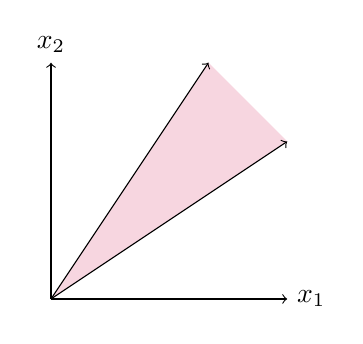
\begin{tikzpicture}
        \draw[->] (0,0) -- (3,0) node[right] {$x_1$};
        \draw[->] (0,0) -- (0,3) node[above] {$x_2$};
        \draw[fill=lightorange, draw=none] (0,0) -- (3,2) -- (2,3) -- cycle;
        \draw[->] (0,0) -- (3,2);
        \draw[->] (0,0) -- (2,3);
    \end{tikzpicture}
\end{center}

\subsubsection{Teorema de Representación de Poliedros}

Todo poliedro $P$ se puede representar como la intersección finita de conos y semiespacios.

\subsubsection{Teorema de No Acotamiento}

Sea $P = \{x \in \mathbb{R}^n: Ax \leq b\}$ no vacío, entonces $P$ es acotado si y solo si $\exists\, h \in \mathbb{R}^n, h \neq 0$ tal que $A h \leq 0$.

\section{Equivalencias}

\subsection{Equivalencia I}

\begin{align*}
    \min \quad f(x) \quad & \sim \quad \max \quad -f(x) \\
    x\,\in D & \qquad x\,\in D
\end{align*}

\subsection{Equivalencia II}

\begin{alignat*}{2}
    \min \quad & f(x) \quad && \sim \quad \min \quad \mu \\
    & && \qquad f(x) \leq \mu \\
    & x\,\in D && \qquad x\,\in D, \mu\,\in \mathbb{R}
\end{alignat*}

\subsection{Equivalencia III}

\begin{alignat*}{2}
    \min \quad & \max \{f_1(x)\dots f_n(x)\} \quad && \sim \quad \min \quad \mu \\
    & && \qquad f_i(x) \leq \mu_i \quad \forall \; i =1\dots r\\
    & x\,\in D && \qquad x\,\in D, \mu\,\in \mathbb{R}^r
\end{alignat*}

\subsection{Equivalencia IV}

\begin{alignat*}{2}
    \min \quad & \sum_{i=1}^{r} f_i(x) \quad && \sim \quad \min \quad \sum_{i=1}^{r}\mu \\
    & && \qquad f_i(x) \leq \mu \quad \forall \; i =1\dots r\\
    & x\,\in D && \qquad x\,\in D, \mu\,\in \mathbb{R}^r
\end{alignat*}

\subsection{Equivalencia V}

\begin{alignat*}{2}
    \min \quad & f(x) \quad && \sim \quad \min \quad g(f(x)) \\
    & && \qquad g \text{ es una función monótona creciente} \\
    & x\,\in D && \qquad x\,\in D
\end{alignat*}

\subsection{Equivalencia VI}

\begin{alignat*}{2}
    \min \quad & \frac{1}{f(x)} \quad && \sim \quad \max \quad f(x) \\
    & && \qquad f(x) > 0 \\
    & x\,\in D && \qquad x\,\in D
\end{alignat*}

\section{Simplex}

El método simplex es un algoritmo iterativo que busca la solución óptima de un problema de programación lineal. La idea es partir de una solución básica factible y moverse a lo largo de las aristas del poliedro de soluciones factibles hasta encontrar la solución óptima.

Se requiere que el problema esté en \textbf{forma estándar}:

\begin{align*}
    \text{Maximizar} \quad & c^T x \\
    \text{Sujeto a} \quad & Ax = b \\
    & x \geq 0
\end{align*}

Con $A$ de rango completo, dado que de otro modo, el problema no tendría solución.


\subsection{Fase II}

\subsubsection{Método para una Iteración}

\begin{enumerate}
    \item Se calculan:
    \begin{align*}
        \overline{b}=B^{-1}b && \pi^T = c_B^T B^{-1}
    \end{align*}
    \item $\overline{b}$ es el valor que tomarían las variables básicas. Así, el \textbf{Criterio de Factibilidad} es:
    \begin{equation*}
        \overline{b} \geq 0
    \end{equation*}

    Si se cumple y un valor es 0, existe una solución degenerada.
    \item Se determina \textbf{Criterio de Optimalidad}:
    \begin{equation*}
        \text{Si } \overline{c}_R^T=c_R^T - \pi^TR \geq 0 \text{, se ha alcanzado la solución óptima}
    \end{equation*}

    Adicionalmente, si algún costo reducido es $0$, entonces el problema tiene soluciones múltiples.
    \item Se verifica el \textbf{Criterio de Entrada}, que determina la variable no básica que tenga los menores costos reducidos. Si el criterio entrega más de un valor, se elige el que tenga el menor índice.
    \begin{equation*}
        \min_{\overline{c}_R^T \geq 0} \{\overline{c}_R^T:j\,\in I_R\} = \overline{c}_e \rightarrow x_e \text{ entra a la base}
    \end{equation*}
    \item Se verifica el \textbf{Criterio de Salida}, que determina la variable básica que debe hacerse cero para llegar al vértice vecino más cercano. Si el criterio de salida entrega más de un valor, se elige arbitrariamente. Si el criterio de salida no entrega ningún valor, el problema es no acotado. Sea $I_B$ el conjunto de índices de las variables básicas, entonces:
    \begin{equation*}
        \min_{a_{ie} > 0} \left\{\frac{\overline{b}_i}{\overline{a}_{ie}} : i\, \in I_B\right\} = \frac{\overline{b}_s}{\overline{a}_{se}} \rightarrow x_s \text{ sale de la base}
    \end{equation*}

\end{enumerate}
\subsection{Fase I}

La fase I del método Simplex utiliza el algoritmo de Simplex para encontrar una solución factible del problema original. Para ello, agrega variables auxiliares que hacen factible una solución que no lo es, al agregar dimensiones al problema.

\begin{enumerate}
    \item Se agregan variables auxiliares en aquellas restricciones que no presentan pivotes para la identidad que genera una solución factible. Para mayor eficiencia, se deja $b\geq 0$ y se agrega un $y_j$ en cada restricción que no presenta pivotes para la identidad.
    \item Se escoge la matriz $B$ del problema como aquella que forma la matriz identidad. En el caso de haber agregado una variable por restricción, la base estará conformada por las variables auxiliares.
    \item Se intenta que las variables auxiliares no sean necesarias para estar en una solución factible del problema original, por lo que se modifica la función objetivo a la suma simple de todas las variables auxiliares que se hayan agregado.
    \item Se comienza a iterar Simplex (como si fuera Fase II) de este nuevo problema auxiliar hasta que el criterio de optimalidad lo indique.
    \item Si la base actual es tal que el valor óptimo de Fase I es igual a 0, entonces esa es la base que se utiliza para comenzar a iterar Fase II del problema original. Si la base actual es tal que el valor óptimo de Fase I es mayor a 0, entonces no existe solución factible para comenzar a iterar Simplex Fase II del problema original.
\end{enumerate}

\section{Análisis de Sensiblidad}

\href{https://youtu.be/oAPScEPsNqY?si=pdlRFEm7N_gvkkHP}{Análisis de Sensibilidad Básico (YT)}

El análisis de sensibilidad se utiliza para estudiar cómo cambia la solución óptima del problema cuando se modifican los parámetros del mismo. Acá se asume una solución óptima $x^*$ con una base óptima $B^*$. A continuación se presentan algunos conceptos importantes relacionados con el análisis de sensibilidad:

\subsection{Cambio en la disponibilidad de los recursos}
Los precios sombra indican el cambio global en la función objetivo al variar en una unidad el lado derecho de una restricción (una componente del vector $b$). Como no se modifica la función objetivo, se verifica si la solución sigue siendo factible.

\begin{align*}
    B^{-1}(b_k + \delta) \geq 0\\
    B^{-1}b_k + B^{-1}\delta \geq 0\\
    B^{-1}_k\delta \geq -B^{-1}b_k\\
    B_k^{-1}\delta \geq -\overline{b}_k
\end{align*}

\subsection{Cambio en los coeficientes de la función objetivo (Costo)}
\subsubsection{Cambio de Coeficiente de una Variable No Básica}

Suponiendo que varía $c_k$ correspondiente a una variable no básica:

\begin{align*}
    (\overline{c}')_j &= \overline{c}_j \\
    (\overline{c}')_k &= {c}_k + \delta - \pi^T R_k \\
    & \overline{c}_k + \delta \geq 0
\end{align*}

Así, el rango para $\delta$ es:

\begin{align*}
    \delta &\geq -\overline{c}_k
\end{align*}

\subsubsection{Cambio de Coeficiente de una Variable Básica}

Suponiendo que varía $c_k$ correspondiente a una variable básica:

\begin{align*}
    c_R^T - (c_B + \Delta)^TB^{-1}R &\geq 0\\
    c_R^T - c_B^TB^{-1}R &\geq \Delta^TB^{-1}R\\
    \overline{c}_R^T &\geq \Delta^TB^{-1}R\\
    \overline{c}_R &\geq \delta n_k
\end{align*}

\subsection{Cambio en los coeficientes de las restricciones}
Si se modifican los coeficientes de las restricciones, es posible que la solución óptima también cambie. El análisis de sensibilidad permite determinar cómo cambia la solución óptima en función de los cambios en los coeficientes de las restricciones.


\subsection{Agregar una variable}

Proceder como si hubiera cambiado un costo no básico, ya que no cambia el tamaño de la base.

\subsection{Agregar una restricción}

Verificar si la solución actual sigue siendo factible. Notar que en este caso la base sí cambia de tamaño.

\section{Dualidad}

Sea el problema primal:

\begin{align*}
    P) \quad z^* = \min z = c^T x \\
    \text{Sujeto a} \quad Ax \geq b \\
    x \geq 0
\end{align*}

El problema dual es:

\begin{align*}
    D) \quad w^* = \max w = b^T y \\
    \text{Sujeto a} \quad A^T y \leq c\\
    y \geq 0
\end{align*}

Para pasar del problema primal al problema dual, se deben seguir los siguientes pasos:

\begin{enumerate}
    \item Por cada restricción $j$ del problema primal se define una variable dual $y_j$.
    \item Los costos del problema dual serán los recursos del problema primal $\mathbf{\overline{b}}$.
    \item Los recursos del problema dual serán los costos del problema primal $\mathbf{c}$.
    \item La matriz $A$ será transpuesta, y las variables que la acompañan serán las variables $\mathbf{y}$.
    \item Los signos de desigualdad de las restricciones y la naturaleza de las variables del problema dual están relacionados directamente con los del primal, según la siguiente tabla:
\end{enumerate}


\begin{center}
    \begin{tabular}{|c|c|}
        \hline
        Min & Max \\
        \hline
        \hline
        Variables & Restricciones \\
        \hline
        $\geq 0$ & $\leq$ \\
        $\leq 0$ & $\geq$ \\
        Irrestrictas & = \\
        \hline
        \hline
        Restricciones & Variables \\
        \hline
        $\geq$ & $\geq$ \\
        $\leq$ & $\leq$ \\
        Irrestrictas & = \\
        \hline
    \end{tabular}
\end{center}

\subsection{Teorema Débil de Dualidad}

Sean $x$ y $y$ soluciones factibles de los problemas primal y dual, respectivamente. Entonces:

\begin{equation*}
    c^T x \geq b^T y
\end{equation*}

Si alguno de los problemas es factible y no acotado, entonces el otro es infactible. Si uno es factible y el otro infactible, entonces el problema que admite solución es no acotado.

\subsection{Lema de Farkas}

Considerando un problema en su forma estándar con una función objetivo $c$ y su dual, entonces:

\begin{equation*}
    Ax=b, x\geq 0 \text{ infactible} \iff \exists y \neq 0: A^T y \leq 0, b^T y > 0
\end{equation*}

\subsection{Teorema Fuerte de Dualidad}

Dado un primal y dual, si uno de los problemas tiene solución óptima, entonces el otro también la tiene, y los valores óptimos son iguales.

\begin{equation*}
    c^T x^* = b^T y^*
\end{equation*}

Se tiene adicionalmente que $y^*=\pi^*$. Es decir, los valores de las variables duales en su óptimo representan los precios sombras de las restricciones respectivas en el primal.

Las holguras del dual son los costos reducidos del primal (y $\geq 0$ en el óptimo). Además, si $x$ no es óptimo para el problema $P$, entonces $y$ no es factible para el problema $D$.

\subsection{Teorema de Holgura Complementaria (THC)}

Para $P$ y $D$ factibles, se tiene que si $x^*$ y $y^*$ son soluciones óptimas de $P$ y $D$, entonces se cumple que:

\begin{align*}
    (c - A^T y^*)^T x^* = 0 \quad & \sim \quad x^*_j \left(c_j - \sum_{i=1}^{m}a_{ij}y_i^*\right)=0, \quad j=1,\ldots,n\\
    (b-Ax^*)^T y^* = 0 \quad & \sim \quad y^*_i \left(b_i - \sum_{j=1}^{n}a_{ij}x_j^*\right)=0, \quad i=1,\ldots,m
\end{align*}

Esto quiere decir que si una restricción no es activa, entonces su variable dual correspondiente es nula. Así, se obtiene:

\begin{center}
    \begin{tabular}{|c|c|}
        \hline
        Primal & Dual \\
        \hline
        \hline
        Variables & Costos reducidos asociados a holguras \\
        \hline
        Holguras & Costos reducidos acodiados a variables \\
        \hline
        Variables Básicas & Costos reducidos de variables no básicas \\
        \hline
        Variables No Básicas & Costos reducidos de variables básicas \\
        \hline
        Múltiples Soluciones & Solución degenerada \\
        \hline
    \end{tabular}
\end{center}
\section{Problemas}

\begin{question}
    Suponga que un problema de Programación Lineal es no acotado. ¿Existe alguna condición que haga que la Fase I de ese problema sea, entonces, no acotada?
\end{question}

\begin{solution}
    No, la Fase I siempre es un problema acotado ya que minimiza la suma de las variables artificiales y estas están acotadas por abajo por cero.
\end{solution}

\begin{question}
    Al resolver un problema de Programación lineal hasta el óptimo se obtiene una solución en donde una variable no básica tiene costo reducido nulo. ¿Significa necesariamente esto que existe otro punto extremo del problema que también es solución optima?
\end{question}

\begin{solution}
    No, no necesariamente. Si bien es cierto que si una variable no básica tiene costo reducido nulo, entonces el problema tiene soluciones múltiples, no necesariamente todas las soluciones múltiples son óptimas.
\end{solution}


\end{document}